
\documentclass{article}
% \documentclass[journal]{IEEEtran}

\usepackage{mlspconf}

\usepackage{cite}
\usepackage{amsmath,amssymb,amsfonts}
\usepackage{algorithmic}
\usepackage{graphicx}
\usepackage{textcomp}
\usepackage{bm}
\usepackage{upgreek}

\usepackage{hyperref}

\usepackage[retainorgcmds]{IEEEtrantools}

\usepackage[nottoc]{tocbibind}


%\linespread{1.3}

%\setcounter{secnumdepth}{3}


\copyrightnotice{978-1-7281-0824-7/19/\$31.00 {\copyright}2019 IEEE}

\toappear{2019 IEEE International Workshop on Machine Learning for Signal Processing, Oct.\ 13--16, 2019, Pittsburgh, PA, USA}


%\graphicspath{ {C:/Users/Paul/Documents/PhD/Dissertation/Documentation/Figures/} }
\graphicspath{ {../Figures/} }


\DeclareMathOperator*{\argmin}{arg\,min}
\DeclareMathOperator*{\argmax}{arg\,max}

\DeclareMathOperator{\xrm}{\mathrm{x}}
\DeclareMathOperator{\Xrm}{\mathrm{X}}
\DeclareMathOperator{\yrm}{\mathrm{y}}
\DeclareMathOperator{\Yrm}{\mathrm{Y}}
\DeclareMathOperator{\Drm}{\mathrm{D}}
\DeclareMathOperator{\nrm}{\mathrm{n}}
\DeclareMathOperator{\nbarrm}{\bar{\mathrm{n}}}
\DeclareMathOperator{\zrm}{\mathrm{z}}

\DeclareMathOperator{\Prm}{\mathrm{P}}
\DeclareMathOperator{\prm}{\mathrm{p}}
\DeclareMathOperator{\Erm}{\mathrm{E}}
\DeclareMathOperator{\Crm}{\mathrm{C}}

\DeclareMathOperator{\Xcal}{\mathcal{X}}
\DeclareMathOperator{\Ycal}{\mathcal{Y}}
\DeclareMathOperator{\Dcal}{\mathcal{D}}
\DeclareMathOperator{\Ncal}{\mathcal{N}}
\DeclareMathOperator{\Zcal}{\mathcal{Z}}
\DeclareMathOperator{\Hcal}{\mathcal{H}}
\DeclareMathOperator{\Fcal}{\mathcal{F}}
\DeclareMathOperator{\Rcal}{\mathcal{R}}
\DeclareMathOperator{\Mcal}{\mathcal{M}}
\DeclareMathOperator{\Scal}{\mathcal{S}}
\DeclareMathOperator{\Pcal}{\mathcal{P}}
\DeclareMathOperator{\Lcal}{\mathcal{L}}

\DeclareMathOperator{\Rbb}{\mathbb{R}}
\DeclareMathOperator{\Nbb}{\mathbb{N}}
\DeclareMathOperator{\Zbb}{\mathbb{Z}}

\DeclareMathOperator{\Dir}{\mathrm{Dir}}
\DeclareMathOperator{\DM}{\mathrm{DM}}
\DeclareMathOperator{\Mult}{\mathrm{Mult}}
\DeclareMathOperator{\DP}{\mathrm{DP}}







\title{Bayesian Regression using Objective and Subjective Dirichlet Priors}

%\name{Paul Rademacher}
%\address{U.S. Naval Research Laboratory}


\twoauthors
  {Paul Rademacher}
	{U.S. Naval Research Laboratory\\Radar Division\\Washington, DC 20375, USA\\paul.rademacher@nrl.navy.mil}
  {Milo\v{s} Doroslova\v{c}ki}
	{The George Washington University\\Department of Electrical and Computer Engineering\\Washington, DC 20052, USA\\
   doroslov@gwu.edu}

%\date{}


\begin{document}

\maketitle


\begin{abstract}
When taking a Bayesian approach to machine learning applications, the performance of the learned function depends critically on how well the prior distribution selected by the designer matches the true data-generating distribution. Dirichlet priors have a number of desirable properties - they lead to analytic posterior distributions given independent observations, have full support over the space of data probability distributions, and can be fully objective or subjective depending on their parameterization. This paper assumes a Dirichlet prior and produces predictive distributions to characterize unobservable random quantities given observed training data. The results are then applied to the most common loss function for regression, the squared-error loss. The optimal Bayes estimator and the corresponding minimum risk are displayed.
\end{abstract}

\begin{keywords}
Bayesian learning, machine learning, regression, estimation, Dirichlet distribution, predictive distribution
\end{keywords}



\section{Introduction}

The success or failure of Bayesian learning methods hinge on how well the prior knowledge imparted by the designer matches reality. The chosen prior distribution over the set of data-generating probability distributions reflects the users confidence that different distributions are responsible for generating the observed/unobserved random elements. If a highly subjective prior is chosen that strongly weights the actual data probability distribution, low risk learning functions are possible even with limited training data; however, if the prior is poorly selected, a good solution will never be achieved. Conversely, an objective prior that treats the different distributions without preference will always be able to adapt will enough training data; if data is limited, however, the learning function may not deliver the required performance.

This work assumes that the joint observed and unobserved data elements are drawn from finite sets. The probability mass function (PMF) generating the data is characterized by a Dirichlet prior. The class of Dirichlet probability density functions (PDF) has the desirable properties of full support over the set of possible data-generating distributions and an analytic posterior distribution for independently and identically distributed data \cite{ferguson}. Furthermore, control of the Dirichlet parameters can enable both truly objective and maximally subjective priors; specifically the uniform distribution over a simplex or an impulsive distribution. 
%The marginal PMF of the training data can be represented with a Dirichlet-Multinomial distribution; new properties will be proven.

After introducing the problem and discussing the relevant data probability distributions, the Bayesian framework will be applied to the most common loss function for regression: the squared error loss function. Algebraic forms of optimal estimators and their corresponding minimum risk will be presented. Specific attention will be given to various asymptotic cases to show the differing performance for objective and subjective Dirichlet priors.











\section{Objective}

Consider an observable random element $\xrm \in \Xcal$ and and unobservable random element $\yrm \in \Ycal$ which are jointly distributed according to an unknown probability distribution $\theta \in \Theta$, such that $\Prm_{\yrm,\xrm | \uptheta}(y,x | \theta) = \theta(y,x)$. 

Also observed is a random sequence of $N$ samples drawn from $\uptheta$, denoted $\Drm = ( \Yrm,\Xrm ) \in \Dcal = \{\Ycal \times \Xcal\}^N$. The $N$ data pairs are identically distributed as $\Prm_{\Drm_n | \uptheta}(y,x | \theta) = \theta(y,x)$ and are conditionally independent from one another and from the novel pair $(\yrm,\xrm)$.

The objective is to design a decision function $f: \Dcal \mapsto \Hcal^{\Xcal}$ which produces a mapping from the space of the observed random element $\xrm$ to a decision space $\Hcal$. The metric guiding the design is a loss function $\Lcal: \Hcal \times \Ycal \mapsto \Rbb_{\geq 0}$ which penalizes the decision $h \in \Hcal$ based on the value of $\yrm$. Introduce the conditional expected loss, or conditional ``risk'',
\begin{equation} \label{eq:risk_cond}
\Rcal_{\Theta}(f ; \uptheta) = \Erm_{\Drm | \uptheta} \bigg[ \Erm_{\yrm,\xrm | \uptheta} \Big[ \Lcal\big( f(\xrm;\Drm),\yrm \big) \Big] \bigg] \;.
\end{equation}

As the model $\uptheta$ is not observed, $\Rcal_{\Theta}$ is not yet a valid objective function for optimization. The designer selects a PDF $\prm_{\uptheta}$ - now the Bayes risk can be formulated as
\begin{IEEEeqnarray}{rCl} \label{eq:risk}
\Rcal(f) & = & \Erm_{\uptheta}\big[ \Rcal_{\Theta}(f ; \uptheta) \big] \\
& = & \Erm_{\yrm,\xrm,\Drm}\big[ \Lcal(f(\xrm;\Drm),\yrm) \big] \nonumber
\end{IEEEeqnarray}
and $\yrm$, $\xrm$, and $\Drm$ are treated as jointly distributed random elements. The optimal learning function is expressed as
\begin{equation} \label{eq:f_opt_xD}
f^*(\xrm;\Drm) = \argmin_{h \in \Hcal} \Erm_{\yrm | \xrm,\Drm}\big[ \Lcal(h,\yrm) \big]
\end{equation}
and the corresponding minimum Bayes risk is
\begin{equation} \label{eq_risk_min}
\Rcal(f^*) = \Erm_{\xrm,\Drm} \left[ \min_{h \in \Hcal} \Erm_{\yrm | \xrm,\Drm}\big[ \Lcal(h,\yrm) \big] \right] \;.
\end{equation}












\section{Probability Distributions}

In this section, the joint PMF $\Prm_{\yrm,\xrm,\Drm}$ is determined using the Dirichlet prior $\prm_{\uptheta}$. Other distributions of interest will be provided, including the training data PMF $\Prm_{\Drm}$ and the predictive distribution $\Prm_{\yrm | \xrm,\Drm}$.



\subsection{Model PDF, $\prm_{\uptheta}$} \label{sec:P_theta}

The Dirichlet PDF for the model random process $\uptheta \in \Theta$ is \cite{bishop}
\begin{IEEEeqnarray}{rCl}
\prm_{\uptheta}(\theta) & = & \beta(\alpha)^{-1} \prod_{y \in \Ycal} \prod_{x \in \Xcal} \theta(y,x)^{\alpha(y,x) - 1} \;,
\end{IEEEeqnarray}
where the user-selected PDF parameters $\alpha : \Ycal \times \Xcal \mapsto \Rbb^+$ are introduced and $\beta$ is the multivariate beta function.

The parameters $\alpha$ controls around which models $\theta$ the PDF concentrates and how strongly. For convenience, introduce the concentration parameter $\alpha_0 \equiv \sum_{y \in \Ycal} \sum_{x \in \Xcal} \alpha(y,x)$. Note that $\Prm_{\yrm,\xrm}(y,x) = \mu_{\uptheta}(y,x) = \alpha(y,x) / \alpha_0$, where $\mu$ denotes the mean function of a random variable.

Of specific interest is how $\prm_{\uptheta}$ changes as the concentration parameter approaches its limiting values. For $\alpha_0 \to \infty$, the PDF concentrates at its mean, resulting in
\begin{IEEEeqnarray}{rCl}
\prm_{\uptheta}(\theta) & = & \delta\left( \theta - \frac{\alpha}{\alpha_0} \right) \;,
\end{IEEEeqnarray}
where $\delta(\cdot)$ represents the Dirac delta function. Conversely, for $\alpha_0 \to 0$, the PDF trends toward
\begin{IEEEeqnarray}{rCl}
\prm_{\uptheta}(\theta) & = & \sum_{y \in \Ycal} \sum_{x \in \Xcal} \frac{\alpha(y,x)}{\alpha_0} \delta\big( \theta - \delta[\cdot,y] \delta[\cdot,x] \big) \;,
\end{IEEEeqnarray}
where $\delta[\cdot,\cdot]$ is the Kronecker delta function. Note that the PDF has support only for the $|\Ycal| |\Xcal|$ models with an $\ell_0$ norm satisfying $\| \theta \|_0 = 1$. 

These trends are demonstrated in Figure \ref{fig:P_theta}. The cardinalities $|\Ycal| = 3$ and $|\Xcal| = 1$ are chosen to enable visualization, despite the implication that $\xrm$ is deterministic. Note that for $\alpha_0=2.99$, $\alpha < 1$ and the PDF values at the boundaries of the domain trend to infinity; this is not captured by the plot color scale.

\begin{figure}
\centering
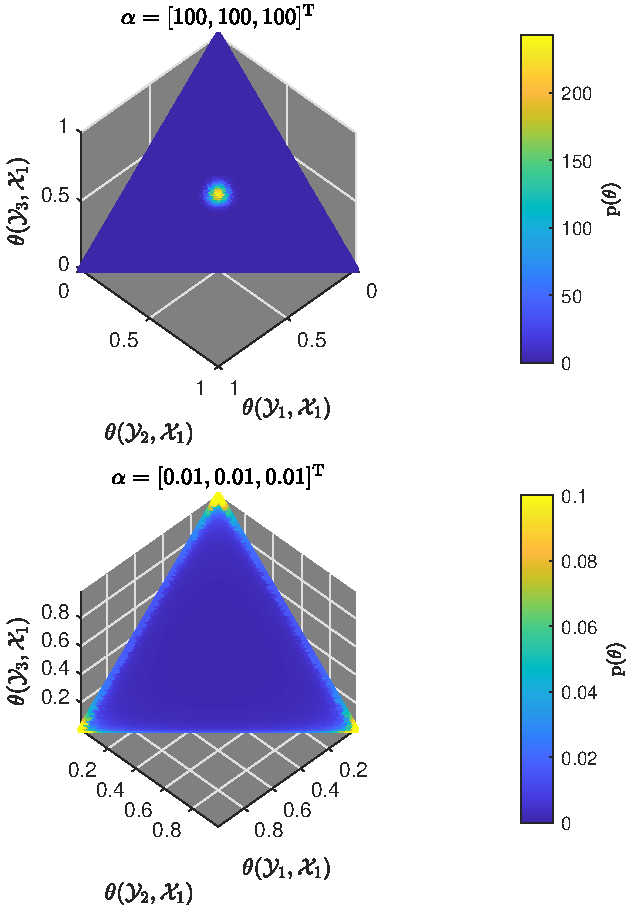
\includegraphics[width=1.0\linewidth]{P_theta.pdf}
\caption{Model prior PDF $\prm_{\uptheta}$ for different concentrations $\alpha_0$}
\label{fig:P_theta}
\end{figure}











\subsection{Training Set PMF, $\Prm_{\Drm}$}

The distribution of the training data $\Drm$ conditioned on the model can be formulated as
\begin{IEEEeqnarray}{rCl}
\Prm_{\Drm | \uptheta}\big( D | \theta \big) & = & \prod_{y \in \Ycal} \prod_{x \in \Xcal} \theta(y,x)^{\bar{N}(y,x;D)} \;,
\end{IEEEeqnarray}
where the dependency on the training data $\Drm$ is expressed though a transform function $\bar{N} : \Dcal \mapsto \bar{\Ncal}$, defined as $\bar{N}(y,x;D) = \sum_{n=1}^N \delta \left[ y,Y_n \right] \delta \left[ x,X_n \right]$. The range of the transform is the function space $\bar{\Ncal} \subset {\Zbb_{\geq 0}}^{\Ycal \times \Xcal}$.


As the conditional distribution $\Prm_{\Drm | \uptheta}$ is of exponential form, it can be readily shown that the marginal distribution of the training data is \cite{minka}
\begin{IEEEeqnarray}{rCl}
\Prm_{\Drm}(D) & = & \beta(\alpha)^{-1} \beta \left(  \alpha + \bar{N}(D) \right) \;.
\end{IEEEeqnarray}


Note that both $\Prm_{\Drm | \uptheta}$ and $\Prm_{\Drm}$ depend on the training data $\Drm$ only through the transform $\bar{N}$; consequently, $\bar{N}(\Drm)$ is a sufficient statistic \cite{bernardo} for the model $\uptheta$. As such, it is useful to define a new random process $\nbarrm \equiv \bar{N}(\Drm) \in \bar{\Ncal}$. 

The cardinality of the random process' domain is $|\bar{\Ncal}| = \Mcal\big( \{N,|\Ycal||\Xcal|-1\} \big)$, where $\Mcal$ is the multinomial coefficient; this can be shown using the stars-and-bars method \cite{feller}. The cardinality of original set is $|\Dcal| = \big( |\Ycal| |\Xcal| \big)^N$; thus $|\bar{\Ncal}| \leq |\Dcal|$ and the sufficient statistic compactly represents the valuable information in the training data. 

It is easily shown that the conditional PMF $\Prm_{\nbarrm | \uptheta}$ is multinomial. As the Dirichlet distribution characterizes the parameters of this multinomial distribution, the marginal PMF of $\nbarrm$ is a Dirichlet-Multinomial distribution \cite{johnson} parameterized by $\alpha$,
\begin{IEEEeqnarray}{rCl}
\Prm_{\nbarrm}(\bar{n}) & = & \Mcal(\bar{n}) \beta(\alpha)^{-1} \beta(\alpha + \bar{n}) \;.
\end{IEEEeqnarray}
The first and second joint moments of $\bar{\nrm}$ are
\begin{IEEEeqnarray}{rCl}
\mu_{\bar{\nrm}}(y,x) & = & N \frac{\alpha(y,x)}{\alpha_0} = N \mu_\uptheta(y,x) 
\end{IEEEeqnarray}
and
\begin{IEEEeqnarray}{L}
\Erm\big[ \bar{\nrm}(y,x) \bar{\nrm}(y',x') \big] \\
= \frac{N}{\alpha_0+1} \Big( (\alpha_0+N) \mu_\uptheta(y,x) \delta[y,y'] \delta[x,x'] \nonumber \\
\qquad \qquad \qquad \qquad \qquad + \alpha_0(N-1) \mu_\uptheta(y,x) \mu_\uptheta(y',x') \Big) \nonumber \;.
\end{IEEEeqnarray}


Again, the data PMF's for minimal and maximal $\alpha_0$ are relevant. For $\alpha_0 \to \infty$, the model PDF $\prm_{\uptheta}$ concentrates at its mean and thus $\bar{\nrm}$ is characterized by a multinomial distribution,
\begin{IEEEeqnarray}{rCl}
\Prm_{\nbarrm}(\bar{n}) & = & \Mcal(\bar{n}) \prod_{y \in \Ycal} \prod_{x \in \Xcal} \left(\frac{\alpha(y,x)}{\alpha_0}\right)^{\bar{n}(y,x)}
\end{IEEEeqnarray}
Conversely, for $\alpha_0 \to 0$, the PMF trends toward
\begin{IEEEeqnarray}{rCl} \label{eq:P_n_lim_zero}
\Prm_{\nbarrm}(\bar{n}) & = & \sum_{y \in \Ycal} \sum_{x \in \Xcal} \frac{\alpha(y,x)}{\alpha_0} \delta\big[ \bar{n} , N \delta[\cdot,y] \delta[\cdot,x] \big]
\end{IEEEeqnarray}
and the training data are identical. 

%Figure \ref{fig:P_nbar_a0} displays the distribution of $\nbarrm$ for $N=10$ and different model concentrations $\alpha_0$. 
%\begin{figure}
%\centering
%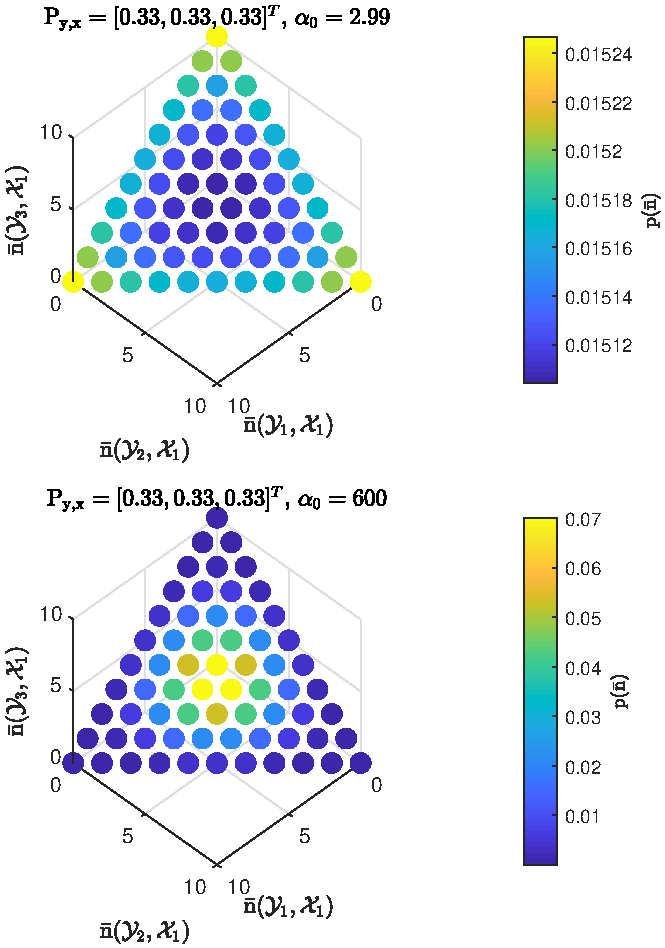
\includegraphics[width=1.0\linewidth]{P_nbar_a0.pdf}
%\caption{$\Prm(\nbarrm)$ for different prior concentrations $\alpha_0$}
%\label{fig:P_nbar_a0}
%\end{figure}





\subsubsection{Aggregation Properties}

Also of importance is the ``marginalized'' random process $\nrm'$, defined as $\nrm'(x) \equiv \sum_{y \in \Ycal} \nbarrm(y,x)$ over the set $\Xcal$. By the aggregation property of Dirichlet-Multinomial functions \cite{johnson}, the new function is distributed as $\nrm' \sim \DM(N,\alpha')$, where $\alpha'(x) = \sum_{y \in \Ycal} \alpha(y,x)$.

Also of interest is the distribution of $\nbarrm$ conditioned on its aggregation $\nrm'$. Using the Dirichlet-Multinomial properties presented in Appendix \ref{app:DM_agg},
\begin{IEEEeqnarray}{L}
\Prm_{\bar{\nrm} | \nrm'}(\bar{n} | n') \\
\quad = \prod_{x \in \Xcal} \left[ \Mcal\big( \bar{n}(\cdot,x) \big) \beta\big( \alpha(\cdot,x) \big)^{-1} \beta\big( \alpha(\cdot,x) + \bar{n}(\cdot,x) \big) \right] \nonumber \;.
\end{IEEEeqnarray}
Observe that conditioning on the aggregation renders the function segments $\nbarrm(\cdot,x)$ independent of one another and that they are also Dirichlet-Multinomial.








\subsection{Predictive PMF, $\Prm_{\yrm | \xrm,\Drm}$}

As shown in Equation \eqref{eq:f_opt_xD}, the decision selected by the optimally designed function depends on the predictive distribution of the unobserved $\yrm$ conditioned on all observable random elements. This PMF will be expressed next.

First observe that since $\Prm_{\Drm | \uptheta}$ is of exponential form, the Dirichlet prior $\prm_{\uptheta}$ is its conjugate prior \cite{theodoridis-ML}; thus, the model posterior PDF given the training data is
\begin{IEEEeqnarray}{L}
\prm_{\uptheta | \Drm}(\theta | D) = \frac{\Prm_{\Drm | \uptheta}(D | \theta) \prm_{\uptheta}(\theta)}{\Prm_{\Drm}(D)} \\
\quad = \beta \left( \alpha + \bar{N}(D) \right)^{-1} \prod_{y \in \Ycal} \prod_{x \in \Xcal} 
\theta(y,x)^{\alpha(y,x) + \bar{N}(y,x;D) - 1} \nonumber \;, 
\end{IEEEeqnarray}
a Dirichlet distribution with parameter function $\alpha + \bar{N}(D)$.

Also, the concentration parameter increases proportionately with increasing volumes of training data; consequently, as $N \to \infty$ the posterior converges to $\prm_{\uptheta | \Drm}(\theta | D) \to \delta\big( \theta - \bar{N}(D) / N \big)$. Thus, as more data is collected, the model can be more positively identified and used to formulate minimum risk decisions. This is a consequence of the full support of the Dirichlet distribution; general priors do not lead to convergent posterior distributions. Conversely, as $\alpha_0 \to \infty$, the prior model certainty is stronger and the posterior trends toward $\prm_{\uptheta | \Drm}(\theta | D) \to \delta( \theta - \alpha / \alpha_0)$, independent of the training data. 


The joint PMF of $\yrm$ and $\xrm$ conditioned on the training data is expressed as \cite{murphy}
\begin{IEEEeqnarray}{rCl}
\Prm_{\yrm,\xrm | \Drm}(y,x | D) & = & \mu_{\uptheta | \Drm}(y,x) \\
& = & \frac{\alpha(y,x) + \bar{N}(y,x;D)}{\alpha_0 + N} \nonumber \;.
\end{IEEEeqnarray}
Next, the predictive distribution is generated via Bayes rule as
\begin{IEEEeqnarray}{rCl}
\Prm_{\yrm | \xrm,\Drm}(y | x,D) & = & \frac{\Prm_{\yrm,\xrm | \Drm}(y,x | D)}{\Prm_{\xrm | \Drm}(x | D)} = \frac{\alpha(y,x) + \bar{N}(y,x;D)}{\alpha'(x) + N'(x;D)} \\
& = & \left(\frac{\alpha'(x)}{\alpha'(x) + N'(x;D)}\right) \Prm_{\yrm | \xrm}(y | x) \nonumber \\
&& \quad + \left(\frac{N'(x;D)}{\alpha'(x) + N'(x;D)}\right) \frac{\bar{N}(y,x;D)}{N'(x;D)} \nonumber \;.
\end{IEEEeqnarray}
The last representation views the distribution as a convex combination of two conditional distributions. The first distribution $\Prm_{\yrm | \xrm}(y | x) = \alpha(y,x) / \alpha'(x)$ is independent of the training data and based on the prior knowledge implied via the model PDF parameter; the second distribution is the conditional empirical PMF and depends on $\Drm$, not on $\alpha$. For both, only those values $\alpha$ and $\Drm$ corresponding to the observed value $\xrm$ influence the distribution. 

The weighting factors are dependent on these values as well. For $N'(x;D) = 0$ or as $\alpha_0 \to \infty$, the PMF trends toward the conditional distribution $\Prm_{\yrm|\xrm}$, which only depends on the model parameter $\alpha$. As the number of training examples increases or as $\alpha_0 \to 0$, $\Prm_{\yrm | \xrm,\Drm}$ trends towards the empirical conditional distribution. 



















\section{Regression and the Squared-Error Loss}

The squared-error (SE) loss function is arguably the most commonly used loss function for regression, or in fact for any estimation problem. This can be attributed to its quadratic form, which enables closed-form expression of the minimizing estimation function $f^*$.

It is assumed that the unobserved random element $\yrm$ is a scalar random variable; that is, $\Ycal \subset \Rbb$. Additionally, the learning function's estimate is allowed to assume real numbers; thus, $\Hcal = \Rbb \supset \Ycal$.

The loss function is defined as
\begin{equation}
\Lcal(h,y) = (h-y)^2 \;.
\end{equation}
Substituting into \eqref{eq:risk}, the Bayes risk for a general estimator is 
\begin{IEEEeqnarray}{rCl} \label{eq:risk_SE}
\Rcal(f) & = & \Erm_{\xrm,\Drm} \bigg[ \Erm_{\yrm | \xrm,\Drm} \Big[ \big( f(\xrm;\Drm)-\yrm \big)^2 \Big] \bigg] \;.
\end{IEEEeqnarray}






\subsection{Optimal Estimate: the Posterior Mean}

To find the optimal estimator, the squared-error loss is substituted into \eqref{eq:f_opt_xD}; note that the objective function is quadratic over the argument $h$. It is easily shown that the function over $h$ is positive-definite; as such, the minimizing decision $h$ is the sole stationary point. Setting the first derivative of the function to zero, the optimal estimate is the expected value of $\yrm$ given the training data and the observed value $\xrm$, such that
\begin{IEEEeqnarray}{rCl} \label{eq:f_opt_SE}
f^*(\xrm;\Drm) & = & \argmin_{h \in \Rbb} \Erm_{\yrm | \xrm,\Drm} \left[ (h-\yrm)^2 \right] = \mu_{\yrm | \xrm,\Drm} \\
& = & \left( \frac{\alpha'(\xrm)}{\alpha'(\xrm) + N'(\xrm;\Drm)} \right) \mu_{\yrm | \xrm} \nonumber \\
&& \quad + \left( \frac{N'(\xrm;\Drm)}{\alpha'(\xrm) + N'(\xrm;\Drm)} \right) \frac{\sum_{n=1}^N \delta\big[ \xrm,\Xrm_n \big] \Yrm_n}{N'(\xrm;\Drm)} \nonumber \;.
\end{IEEEeqnarray}

The optimal estimate is interpreted as a convex combination of two separate estimates - the expected value of $\yrm$ conditioned on the observed $\xrm$ and the mean of the training values $\Yrm_n$ which have a value $\Xrm_n$ matching the observed value $\xrm$. The weighting factors are the same as those of $\Prm_{\yrm | \xrm,\Drm}$; thus, stronger prior information (larger $\alpha'(x)$) provides more weight to the estimate $\mu_{\yrm|\xrm}$ and more voluminous training data puts emphasis on the empirical conditional mean.

Another interesting form for the optimal estimator is $f^*(\xrm;\Drm) = \Erm_{\uptheta | \xrm,\Drm} \left[ \mu_{\yrm | \xrm,\uptheta} \right]$. If the model $\uptheta$ were known, then the expectation $\mu_{\yrm | \xrm,\uptheta}$ would be optimal; instead, all such estimates are weighted and combined via the expectation over the model posterior PDF $\prm_{\uptheta | \xrm,\Drm}$.







\subsection{Minimum Risk: the Expected Posterior Variance}

Substituting the optimal estimator \eqref{eq:f_opt_SE} into Equation \eqref{eq:risk_SE}, the minimum Bayes risk is the expected conditional variance
\begin{IEEEeqnarray}{rCl}
\Rcal(f^*) & = & \Erm_{\xrm,\Drm} \left[ \Sigma_{\yrm | \xrm,\Drm} \right] \\
& = & \Erm_{\xrm,\uptheta} \left[ \Sigma_{\yrm | \xrm,\uptheta} \right] + \Erm_{\xrm,\Drm} \left[ \Crm_{\uptheta | \xrm,\Drm} \left[ \mu_{\yrm | \xrm,\uptheta} \right] \right] \nonumber \;,
\end{IEEEeqnarray}
where $\Sigma$ is the covariance function and the operator $C$ computes the covariance of a function of a random variable. The second formula is of interest. The first term is the expected irreducible risk; the second term is the expected variance of the clairvoyant estimate $\mu_{\yrm | \xrm,\uptheta}$, where the variance is evaluated with respect to the model posterior PDF $\prm_{\uptheta | \xrm,\Drm}$

Using the sufficient statistic $\nbarrm \equiv \bar{N}(\Drm)$, the minimum risk can also be represented as $\Erm_{\xrm,\nbarrm} \left[ \Sigma_{\yrm | \xrm,\nbarrm} \right]$. Decompose the conditional variance as
\begin{IEEEeqnarray}{rCl}
\Sigma_{\yrm | \xrm,\nbarrm} & = & \Erm_{\yrm | \xrm,\nbarrm}[\yrm^2] - {\mu_{\yrm | \xrm,\nbarrm}}^2 
\end{IEEEeqnarray}
and assess the expected values of these terms separately. The first term is 
\begin{IEEEeqnarray}{L}
\Erm_{\xrm,\nbarrm} \left[ \Erm_{\yrm | \xrm,\nbarrm}[\yrm^2] \right] = \Erm_{\xrm} \big[ \Erm_{\yrm | \xrm} [ \yrm^2 ] \big] \;,
\end{IEEEeqnarray}
where the expectation over $\xrm$ is performed using $\Prm_{\xrm} = \alpha'/\alpha_0$. As proven in Appendix \ref{app:SE_proof}, the second term is
\begin{IEEEeqnarray}{L}
\Erm_{\xrm,\nbarrm} \Big[ {\mu_{\yrm | \xrm,\nbarrm}}^2 \Big] \nonumber \\
\quad = \Erm_{\xrm} \left[ \frac{N \Erm_{\yrm|\xrm}[\yrm^2] + \big( \alpha_0 \alpha'(\xrm) + N \alpha'(\xrm) + \alpha_0 \big) {\mu_{\yrm|\xrm}}^2 }{(\alpha_0+N) \big( \alpha'(\xrm)+1 \big)} \right] \nonumber \;.
\end{IEEEeqnarray}


Combining, the mininum Bayes risk is
\begin{IEEEeqnarray}{L}
\Rcal(f^*) = \Erm_{\xrm,\nbarrm} \left[ \Erm_{\yrm | \xrm,\nbarrm}[\yrm^2] - {\mu_{\yrm | \xrm,\nbarrm}}^2 \right] \\
= \Erm_{\xrm} \left[ \frac{\Prm_{\xrm}(\xrm) + (\alpha_0+N)^{-1}}{\Prm_{\xrm}(\xrm) + \alpha_0^{-1}} \Sigma_{\yrm | \xrm} \right] \nonumber \;.
\end{IEEEeqnarray}
The risk is a convex combination of scaled conditional variances for the different PMF's $\Prm_{\yrm | \xrm}$. The convex coefficients are values from the prior marginal distribution $\Prm_{\xrm}$. 

The scaling factor for each term $\Sigma_{\yrm | \xrm}$ depends on the marginal PMF value $\Prm_{\xrm}(\xrm)$, as well as on the prior concentration $\alpha_0$ and the number of training samples $N$. Observe that with no training data ($N = 0$), the scaling factor becomes unity and the risk is $\Rcal(f^*) = \Erm_{\xrm} \left[ \Sigma_{\yrm | \xrm} \right]$. Conversely, as $N \to \infty$, the Bayes risk is $\Rcal(f^*) = \Erm_{\xrm} \left[ \frac{\Prm_{\xrm}(\xrm)}{\Prm_{\xrm}(\xrm) + \alpha_0^{-1}} \Sigma_{\yrm | \xrm} \right] = \Erm_{\xrm,\uptheta} \left[ \Sigma_{\yrm | \xrm,\uptheta} \right]$. Also, as the model concentration parameter $\alpha_0 \to 0$, the risk trends to zero (for $N > 0$); as $\alpha_0 \to \infty$, the risk trends toward $\Erm_{\xrm} \left[ \Sigma_{\yrm | \xrm} \right]$.


\subsubsection{Examples}

To illustrate these trends, explicitly define the sets $\Ycal = \{ i/M_{\yrm} : i = 0,\ldots,M_{\yrm}-1 \}$ and $\Xcal = \{ i/M_{\xrm} : i = 0,\ldots,M_{\xrm}-1 \}$. First assume that the conditional variance $\Sigma_{\yrm | \xrm}$ is independent of $\xrm$; in this case, the squared-error becomes the conditional variance scaled by a factor dependent on the marginal distribution $\Prm_{\xrm}$, such that $\Rcal(f^*) = \Sigma_{\yrm | \xrm} \Erm_{\xrm} \left[ \frac{\Prm_{\xrm}(\xrm) + (\alpha_0+N)^{-1}}{\Prm_{\xrm}(\xrm) + \alpha_0^{-1}} \right]$.  Figures \ref{fig:Risk_SE_Dir_IO_N_leg_a0} and \ref{fig:Risk_SE_Dir_IO_a0_leg_N} display how the risk changes with $N$ and $\alpha_0$ when $\Prm_{\yrm|\xrm}$ and $\Prm_{\xrm}$ are fixed.

\begin{figure}
\centering
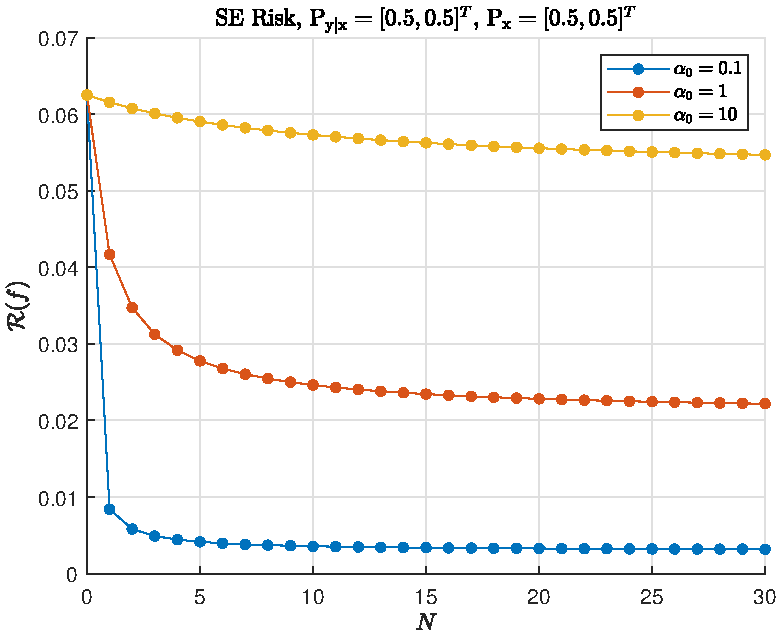
\includegraphics[width=1.0\linewidth]{Risk_SE_Dir_IO_N_leg_a0.pdf}
\caption{Optimal SE Risk for different training set sizes $N$}
\label{fig:Risk_SE_Dir_IO_N_leg_a0}
\end{figure}

\begin{figure}
\centering
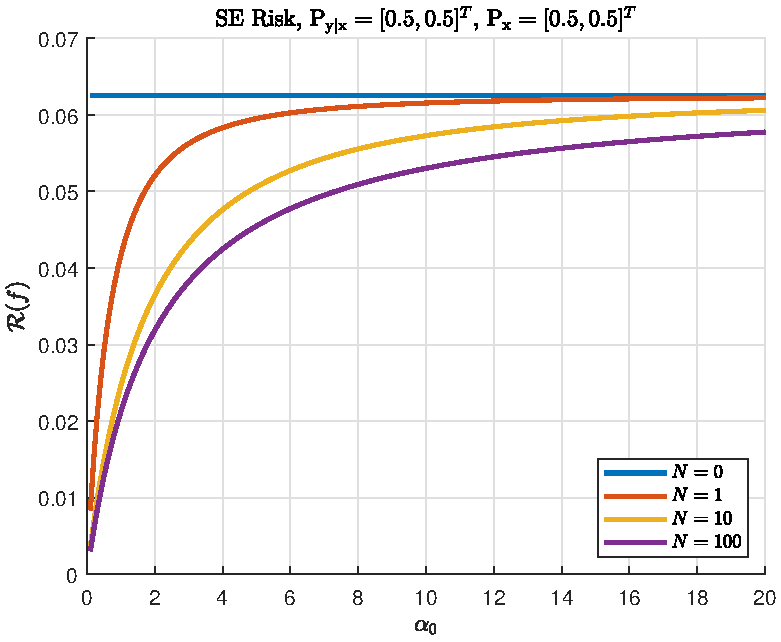
\includegraphics[width=1.0\linewidth]{Risk_SE_Dir_IO_a0_leg_N.pdf}
\caption{Optimal SE Risk for different prior concentrations $\alpha_0$}
\label{fig:Risk_SE_Dir_IO_a0_leg_N}
\end{figure}

It may not seem intutitve for the risk to decrease when $\alpha_0$ is smaller -- the variance of the model $\uptheta$ increases and the prior knowledge is less definitive. This is a result of the Dirichlet PDF weight shifting towards the $|\Ycal||\Xcal|$ models which have $\ell_0$ norms satisfying $\| \theta \|_0 = 1$. Although these PMF's are maximally separated (and uncorrelated), they all have zero variance and thus zero risk. The optimal learner will simply use the empirical distribution supplied via the training data - this allows exact identification of $\uptheta$ with a single training pair and leads to predictions that match the single element represented in $\Yrm$.

It is also informative to visualize how the minimum squared-error changes for fixed volume of training data $N$ and a fixed prior concentration $\alpha_0$. Consider the effect of the marginal distribution $\Prm_{\xrm}$. Figure \ref{fig:Risk_SE_Dir_IO_Px_N_10_a0_1} demonstrates how the risk changes with this marginal PMF. Observe that the risk is maximal at the distributions satisfying $\| \Prm_{\xrm} \|_0 = 1$; the scaling factor for the conditional variance $\Sigma_{\yrm | \xrm}$ becomes $\frac{1 + (\alpha_0+N)^{-1}}{1 + \alpha_0^{-1}}$. Conversely, for $\Prm_{\xrm} = 1/|\Xcal|$ the scaling factor becomes $\frac{|\Xcal|^{-1} + (\alpha_0+N)^{-1}}{|\Xcal|^{-1} + \alpha_0^{-1}}$ and the risk is minimal. 

%Figures \ref{fig:Risk_SE_Dir_IO_N_leg_Px} and \ref{fig:Risk_SE_Dir_IO_a0_leg_Px} show how different marginals $\Prm(\xrm)$ affect the risk as a function of $N$ and $\alpha_0$, respectively.

\begin{figure}
\centering
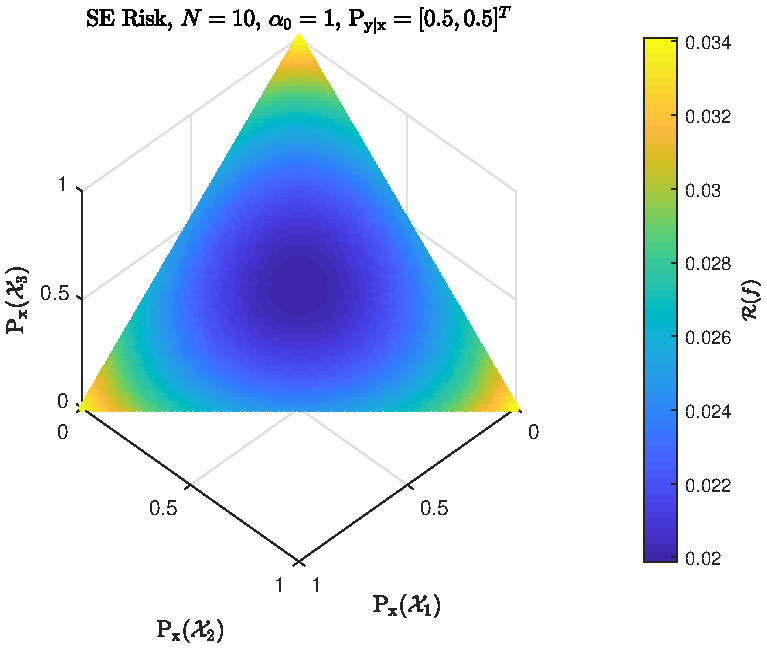
\includegraphics[width=1.0\linewidth]{Risk_SE_Dir_IO_Px_N_10_a0_1.pdf}
\caption{Optimal SE Risk for different PMF's $\Prm_{\xrm}$}
\label{fig:Risk_SE_Dir_IO_Px_N_10_a0_1}
\end{figure}

%\begin{figure}
%\centering
%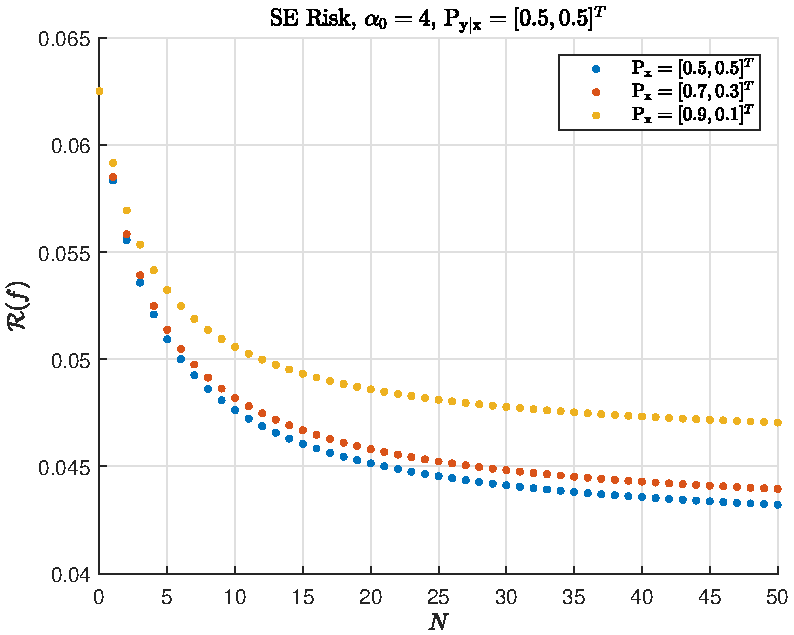
\includegraphics[width=1.0\linewidth]{Risk_SE_Dir_IO_N_leg_Px.pdf}
%\caption{Optimal SE Risk for different training set sizes $N$}
%\label{fig:Risk_SE_Dir_IO_N_leg_Px}
%\end{figure}
%
%\begin{figure}
%\centering
%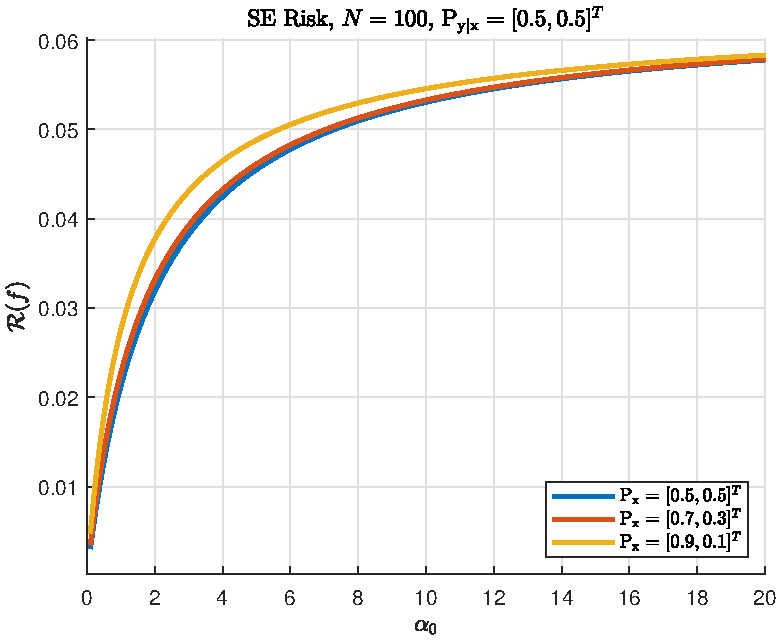
\includegraphics[width=1.0\linewidth]{Risk_SE_Dir_IO_a0_leg_Px.pdf}
%\caption{Optimal SE Risk for different prior concentrations $\alpha_0$}
%\label{fig:Risk_SE_Dir_IO_a0_leg_Px}
%\end{figure}



\section{Conclusions}

This paper has assumed a Dirichlet prior for Bayesian learning, established relevant distributions, and applied the framework to the regression application. Closed-forms have been provided for the optimal estimation function and the minimum Bayes risk. Analysis and graphic examples highlight interesting trends in the expected squared-error as a function of the Dirichlet prior distribution parameters. Most notably, Dirichlet priors with smaller concentration parameters (and thus larger covariance) lead to optimal estimators with lower risk. Future work will explore this consequence of Dirichlet prior selection and show that it does not hold for general prior distributions.








\appendix


\section{Dirichlet-Multinomial random process conditioned on its aggregation} 
\label{app:DM_agg}

A defining characteristic of a Dirichlet-Multinomial random process is that its aggregations are also Dirichlet-Multinomial \cite{johnson}. Consider a DM random process $\bar{\nrm} \sim \DM(N,\alpha)$ over the set $\Ycal$. Define an arbitrary partition of $\Ycal$: $\left\{ \ldots,\Scal(z),\ldots \right\}$, $z \in \Zcal$; the transformed random process $\nrm'(z) \equiv \sum_{y \in \Scal(z)} \bar{\nrm}(y)$ is neccessarily Dirichlet-Multinomial with parameterizing function $\alpha'(z) = \sum_{y \in \Scal(z)} \alpha(y)$.

It can be shown that conditioned on the aggregation $\nrm'$, the segments $\big\{ \bar{\nrm}(y) : y \in \Scal(z) \big\}$ of the original random process become independent Dirichlet-Multinomial random processes, such that
\begin{IEEEeqnarray}{L}
\Prm_{\bar{\nrm} | \nrm'}(\bar{n} | n') = \frac{\Prm_{\bar{\nrm}}(\bar{n})}{\Prm_{\nrm'}(n')} \Prm_{\nrm' | \bar{\nrm}}(n' | \bar{n}) \\ 
\quad = \frac{\Mcal(\bar{n}) \beta(\alpha)^{-1} \beta(\alpha+\bar{n})}{\Mcal(n') \beta(\alpha')^{-1} \beta(\alpha'+n')} \nonumber \\
\quad = \left( \prod_{z \in \Zcal} \frac{\Gamma\big( \alpha'(z)+n'(z) \big)}{n'(z)! \Gamma\big( \alpha'(z) \big)} \right)^{-1} \left( \prod_{y \in \Ycal} \frac{\Gamma\big( \alpha(y)+\bar{n}(y) \big)}{\bar{n}(y)! \Gamma\big( \alpha(y) \big)} \right) \nonumber \\
\quad = \prod_{z \in \Zcal} \left[ \frac{n'(z)! \Gamma\big( \alpha'(z) \big)}{\Gamma\big( \alpha'(z)+n'(z) \big)} \prod_{y \in \Scal(z)} \frac{\Gamma\big( \alpha(y)+\bar{n}(y) \big)}{\bar{n}(y)! \Gamma\big( \alpha(y) \big)} \right] \nonumber \;,
\end{IEEEeqnarray}
over domain $\bar{\nrm} \in \left\{ {\Zbb_{\geq 0}}^{\Ycal} : \sum_{y \in \Scal(z)} \bar{n}(y) = \nrm'(z), \quad \forall z \in \Zcal \right\}$. 





\section{Formulation of $\Erm_{\xrm,\nbarrm} \Big[ {\mu_{\yrm | \xrm,\nbarrm}}^2 \Big]$} 
\label{app:SE_proof}

The expected value of the conditional squared mean can be determined as
\begin{IEEEeqnarray}{L}
\Erm_{\xrm,\nbarrm} \Big[ {\mu_{\yrm | \xrm,\nbarrm}}^2 \Big] =
\sum_{\bar{n} \in \bar{\Ncal}} \sum_{x \in \Xcal} \Prm_{\xrm,\nbarrm}(x,\bar{n}) \left( \sum_{y \in \Ycal} y \Prm_{\yrm | \xrm,\nbarrm}(y | x,\bar{n}) \right)^2 \\
= \sum_{x \in \Xcal} \sum_{y \in \Ycal} y \sum_{y' \in \Ycal} y' \Erm_{\nbarrm} \Big[ \Prm_{\yrm,\xrm | \nbarrm}(y,x | \nbarrm) \Prm_{\yrm | \xrm,\nbarrm}(y' | x,\nbarrm) \Big] \nonumber \\
= \sum_{x \in \Xcal} \sum_{y \in \Ycal} y \sum_{y' \in \Ycal} y' \Erm_{\nrm'} \left[ \frac{\Erm_{\nbarrm | \nrm'} \left[ \big( \alpha(y,x)+\bar{\nrm}(y,x) \big) \big(\alpha(y',x)+\bar{\nrm}(y',x) \big) \right]}{(\alpha_0+N) \big(\alpha'(x) + \nrm'(x) \big)} \right] \nonumber \\
= \sum_{x \in \Xcal} \frac{\Erm_{\nrm'} \Big[ \nrm'(x) \Erm_{\yrm|\xrm}[\yrm^2](x) + \alpha'(x) \big( \alpha'(x) + \nrm'(x) + 1 \big) \mu_{\yrm|\xrm}(x)^2 \Big]}{(\alpha_0+N) \big(\alpha'(x) + 1 \big)} \nonumber \\
= \Erm_{\xrm} \left[ \frac{N \Erm_{\yrm|\xrm}[\yrm^2] + \big( \alpha_0 \alpha'(\xrm) + N \alpha'(\xrm) + \alpha_0 \big) {\mu_{\yrm|\xrm}}^2 }{(\alpha_0+N) \big( \alpha'(\xrm)+1 \big)} \right] \nonumber \;.
\end{IEEEeqnarray}
The formulation uses the statistical characterization of the aggregation, $\nrm' \sim \DM(N,\alpha')$; also used is the property that the Dirichlet-Multinomial random process $\nbarrm$ conditioned on its aggregation $\nrm'$ yields independent conditional DM functions $\bar{\nrm}(\cdot,x) | \nrm'(x) \sim \DM\big( \nrm'(x),\alpha(\cdot,x) \big)$.




\bibliographystyle{IEEEbib}
\bibliography{{../References/phd_bib}}


\end{document}


























